% Activate the following line by filling in the right side. If for example the name of the root file is Main.tex, write
% "...root = Main.tex" if the chapter file is in the same directory, and "...root = ../Main.tex" if the chapter is in a subdirectory.
 
%!TEX root =  

\chapter[Systematic Uncertainties]{Systematic Uncertainties}

The last step in computing a result in experimental physics involves identifying
and quantifying sources of systematic error.  Systematic errors arise from calibration
errors, data/MC disagreement, detector uncertainty, noise, and other sources
that do not decrease as the overall dataset size increases.  

Since we use a data-driven background estimate, most of the systematic errors
are only relevant for the signal shape and normalization, which we study using 
MC simulations.  For example, $b$-tagging systematics, jet energy systematics, 
and trigger turn-on systematics only apply to signal and not to background.  
However, the shape extrapolation from the \textit{bbanti} control region to the
\textit{bbb} signal region is one important source of background uncertainty;
we validate the extrapolation and compute systematic errors for it using QCD MC simulations.

\section{Background Shape Extrapolation Systematics}
\label{sec:background_syst}
The background shape is data-driven, since it comes from the \textit{bbanti} $m^{'}_{bb}$ distribution in data, but the
extrapolation from the \textit{bbanti} background control region to the \textit{bbb} signal region needs to be validated
in MC. In general, these validation studies show clearly that the $m^{'}_{bb}$ shape agrees closely between the
\textit{bbanti} and \textit{bbb} regions (validation plots can be found in Section~\ref{sec:bb_qcd_mc}), but any small differences must
be estimated as systematics.

In order to compare the shapes, we calculate the ratio between the $m^{'}_{bb}$ distributions in the \textit{bbb} and
\textit{bbanti} samples in QCD MC. Then we fit these ratios with a linear function, looking at the slope of the
line to see if it is significantly different from zero, indicating a systematic shape difference. These fitted ′
ratio plots can be seen in Figure~\ref{fig:shape_checks_bg}.  Clearly the largest shape uncertainty arises in
the 5 jet category; we believe that in the higher-jet categories (four-jet and five-jet) there is a combinatorial
effect where several jets are available to provide the ``third'' $b$-tag required for the event to be classified
in the \textit{bbb} category and that has a slight effect on the $m^{'}_{bb}$ distribution relative to the
three-jet category.


\begin{figure}
    \center
  \includegraphics[width=0.3\linewidth]{Systematics/images/shape_check_mbb_bbb_3jets_extendedbAbb_450_rotated.eps}
  \includegraphics[width=0.3\linewidth]{Systematics/images/shape_check_mbb_bbb_4jets_extendedbAbb_450_rotated.eps}
  \includegraphics[width=0.3\linewidth]{Systematics/images/shape_check_mbb_bbb_5jets_extendedbAbb_450_rotated.eps}
  \includegraphics[width=0.3\linewidth]{Systematics/images/shape_check_mbb_bbb_3jets_extendedbAbb_500_rotated.eps}
  \includegraphics[width=0.3\linewidth]{Systematics/images/shape_check_mbb_bbb_4jets_extendedbAbb_500_rotated.eps}
  \includegraphics[width=0.3\linewidth]{Systematics/images/shape_check_mbb_bbb_5jets_extendedbAbb_500_rotated.eps}
  \includegraphics[width=0.3\linewidth]{Systematics/images/shape_check_mbb_bbb_3jets_extendedbAbb_550_rotated.eps}
  \includegraphics[width=0.3\linewidth]{Systematics/images/shape_check_mbb_bbb_4jets_extendedbAbb_550_rotated.eps}
  \includegraphics[width=0.3\linewidth]{Systematics/images/shape_check_mbb_bbb_5jets_extendedbAbb_550_rotated.eps}
  \caption{The ratio of the $m^{'}_{bb}$ distributions in QCD MC simulations of \textit{bbanti}
  and \textit{bbb} events, fitted with a linear function, for the 3-jet, 4-jet and 5-jet categories for 
  $m_A$=450, 500, and 550 GeV.
  The slope and intercept of the best fit line are printed on the plots, along with their error
  and the $\chi^2$ and number of degrees of freedom of the fit.\label{fig:shape_checks_bg_1}}    
\end{figure}                                                                                                                        
\begin{figure}
    \center
  \includegraphics[width=0.3\linewidth]{Systematics/images/shape_check_mbb_bbb_3jets_extendedbAbb_600_rotated.eps}
  \includegraphics[width=0.3\linewidth]{Systematics/images/shape_check_mbb_bbb_4jets_extendedbAbb_600_rotated.eps}
  \includegraphics[width=0.3\linewidth]{Systematics/images/shape_check_mbb_bbb_5jets_extendedbAbb_600_rotated.eps}
  \includegraphics[width=0.3\linewidth]{Systematics/images/shape_check_mbb_bbb_3jets_extendedbAbb_650_rotated.eps}
  \includegraphics[width=0.3\linewidth]{Systematics/images/shape_check_mbb_bbb_4jets_extendedbAbb_650_rotated.eps}
  \includegraphics[width=0.3\linewidth]{Systematics/images/shape_check_mbb_bbb_5jets_extendedbAbb_650_rotated.eps}
  \includegraphics[width=0.3\linewidth]{Systematics/images/shape_check_mbb_bbb_3jets_extendedbAbb_700_rotated.eps}
  \includegraphics[width=0.3\linewidth]{Systematics/images/shape_check_mbb_bbb_4jets_extendedbAbb_700_rotated.eps}
  \includegraphics[width=0.3\linewidth]{Systematics/images/shape_check_mbb_bbb_5jets_extendedbAbb_700_rotated.eps}
  \includegraphics[width=0.3\linewidth]{Systematics/images/shape_check_mbb_bbb_3jets_extendedbAbb_800_rotated.eps}
  \includegraphics[width=0.3\linewidth]{Systematics/images/shape_check_mbb_bbb_4jets_extendedbAbb_800_rotated.eps}
  \includegraphics[width=0.3\linewidth]{Systematics/images/shape_check_mbb_bbb_5jets_extendedbAbb_800_rotated.eps}
  \caption{The ratio of the $m^{'}_{bb}$ distributions in QCD MC simulations of \textit{bbanti}
  and \textit{bbb} events, fitted with a linear function, for the 3-jet, 4-jet and 5-jet categories for 
  $m_A$=600-800 GeV.
  The slope and intercept of the best fit line are printed on the plots, along with their error
  and the $\chi^2$ and number of degrees of freedom of the fit.\label{fig:shape_checks_bg_2}}    
\end{figure}

There are two systematic scenarios that we explore.  The first is to take the central values of the
slopes of these fits, and use that as a correction factor for varying the \textit{bbb} PDF
relative to \textit{bbanti}.  Then the statistical error on the slope is taken as a systematic error.
The second treatment takes the sum in quadrature of the slope and the error on the slope is
taken as a systematic error, which of course leads to a larger systematic overall but allows for
more uncertainty on the background MC modeling and whether it precisely matches the data.


\subsection{Shape Correction with Systematic Based on Statistical Errors of Ratio Fit}

\subsection{Systematic Based on Slope Plus Statistical Error}
For a second study of the background shape systematic error, 
we assign a systematic variation based on the quadratic sum of the slope of the best
fit line, and the error on the slope. This is done separately in each of the jet categories.
This uncertainty is assigned as a reweighting to the \textit{bbanti} $m^{'}_{bb}$ distribution
when we extrapolate it to the \textit{bbb} signal region; the reweighted distributions can be
seen in Figure~\ref{fig:shape_error_bg}.
\begin{figure}
    \center
  \includegraphics[width=0.45\linewidth]{Systematics/mbb_shape_systematic_bAbb_700_3jets_quad_err.eps}
  \includegraphics[width=0.45\linewidth]{Systematics/mbb_shape_systematic_bAbb_700_4jets_quad_err.eps}
  \includegraphics[width=0.45\linewidth]{Systematics/mbb_shape_systematic_bAbb_700_5jets_quad_err.eps}
  \caption{The \textit{bbanti} $m^{'}_{bb}$ distribution in data, for the nominal case (i.e. no 
  adjustments made) and with a systematic variation applied based on the shape differences between \textit{bbanti}
  and \textit{bbb}, as quantified in Figure~\ref{fig:shape_checks_bg}.\label{fig:shape_error_bg}}
\end{figure}                                                                                                                        
 
In order to estimate the effect of this systematic on the final sensitivity, we take the
reweighted \textit{bbanti} distributions and send them through the nominal fitting procedure\footnote{the 
nominal fit makes the assumption of the same background shape in the \textit{bbb}, \textit{bbloose},
and \textit{bbanti}}, 
and take the variation in the signal cross section returned by the fit as a systematic error.

We find that, since the slope of the \textit{bbb} to \textit{bbanti} ratio can change
based on the signal mass point\footnote{a result of statistical variations and different
rotations for each signal mass point}, the size of the resulting systematic can vary as well.
For example, we find that for the 600 GeV mass point, the best fit to the ratios returns a 
slope very close to zero, which propagates through to a very small associated systematic error
\footnote{recall that the size of the variation is the sum in quadrature of the slope and the
statistical error on the slope, so even a slope of zero will still have a non-zero variation
because of the statistical error}.  In order to be conservative, we examine the 
associated systematic errors for a number of mass points (550-800 GeV) and find 
the largest effect of this systematic is 0.29 pb (at 650 GeV) so we assign 0.3 pb
as the background shape systematic for all mass points above 500 GeV.  For the lower mass
points, 450 and 500 GeV, we find larger background shape systematic effects, so 
we assign uncertainties to the signal cross section of 4.0 pb at 450 GeV, and 1.2 pb at 500 GeV. 
The systematic that is assigned for each mass point is in Table~\ref{tab:bkg_shape_syst}.

\begin{table}
    \center
    \caption{The variation in the signal cross section returned by the fit when the 
    background shape is varied in \textit{bbb} relative to \textit{bbanti} by the amounts
    quantified in Figures~\ref{fig:shape_checks_bg_1} and~\ref{fig:shape_checks_bg_2}.
    \label{tab:bkg_shape_syst}}
    \begin{tabular}{c c c} \hline \hline
        mass point & variation on signal $\sigma$ [pb] returned by fit  & systematic error assigned  \\ \hline
        450 & 3.99 & 4.0\\
        500 & 1.18 & 1.2\\
        550 & 0.15 & 0.3 \\
        600 & 0.04 & 0.3\\
        650 & 0.29 & 0.3\\
        700 & 0.16 & 0.3\\
        800 & 0.30 & 0.3\\
    \end{tabular}
\end{table}


 

\section{Trigger $p_T$ Efficiency}
\label{sec:trigger_syst}

The trigger can introduce systematic effects that must be quantified as uncertainties; 
this can happen in two ways on this analysis.  Since the trigger efficiency is estimated
for signal using MC simulations, it is possible that detector mismodelings in the MC 
simulation process can over- or under-estimate the trigger efficiency as a function 
of the $p_T$ of the jets in the event.  We call this the trigger $p_T$ efficiency,
and we estimate and correct for it by parameterizing the turn-on curve with a logistic
function, and using the ratio of the function between data and MC to calculate and 
apply scale factors that get applied to the MC events falling in the turn-on curve.  
The second source of trigger mismodeling comes from the online $b$-tag that is
included in the trigger, but because of correlations between the online and offline tagging,
we estimate this uncertainty as part of the $b$-tagging sytematic (Section ~\ref{sec:SF}).


The general idea behind the trigger turn-on curve is that the overall trigger efficiency
is more volatile if one or both of the relevant jets are near the $p_T$ thresholds.
Since there are two jets in the EF\_2b35\_loose\_j145\_j35\_a4tchad trigger, with thresholds
of 145 and 35 GeV respectively, events with jets near these values should be assessed
for systematic errors.  However, since this is a multi-object trigger (requiring $b$-tags
in addition to the two jets), the efficiency for a given event can be a complex function
of the $p_T$ of the leading jet, the second jet, and the $b$-tagging characteristics of
the jets in the event.  In order to factorize out these effects, we place tight offline
cuts on all objects in the trigger \textit{except} the object under examination. For example, 
to compute the trigger turn-on curve for the leading jet, we place the following cuts before
computing any efficiencies: 
\begin{itemize}
    \item at least 60 GeV $p_T$ for the second jet
    \item two jets in the event must pass L2 and EF $b$-tags
\end{itemize}

These cuts effectively remove inefficiencies due to the second jet or the $b$-tagging,
since the second jet $p_T$ cut (60 GeV) is well into the efficiency plateau for that
jet, and the requirement of two jets being $b$-tagged online removes events where the
jet $p_T$ is high enough, but the event fails to trigger because of the $b$-tagging requirement.  
In this discussion the same algorithm is applied to quantify
the trigger turn-on of both the leading and sub-leading jet, but for brevity we will
refer only to the leading jet.  The parameterized turn-on curves for the leading and 
sub-leading jets in signal MC and data can be found in Figure~\ref{fig:trigger_turn_on_1}.

For signal MC we can then compute the efficiency as a function of the leading jet $p_T$ by
examining the leading jet $p_T$ of events that both do and do not pass the trigger.
Residual inefficiencies remaining from the second jet $p_T$, and the $b$-tagging requirements,
would show up in the form of the distribution plateauing slightly below 100\% efficiency;
the logistic function will identify the plateau efficiency and the residual error can be corrected when
computing the trigger efficiency for a given jet $p_T$.  The logistic function used for 
fitting has the mathematical form $\epsilon = \frac{b}{1+e^{c-a*p_T}}$.  The values found
by ROOT for the parameters of this function are as follows:

\scriptsize
\begin{verbatim}
---------- turn-on for j145 jet -----------
 FCN=485.311 FROM MIGRAD    STATUS=CONVERGED     229 CALLS         230 TOTAL
 EDM=2.12809e-08    STRATEGY= 1      ERROR MATRIX ACCURATE 
 EXT PARAMETER                                   STEP         FIRST   
 NO.   NAME      VALUE            ERROR          SIZE      DERIVATIVE 
 1  a           7.02887e+01   4.79927e-01   1.69260e-04  -1.12470e-02
 2  b           9.32043e-01   7.98882e-04   8.34460e-06   1.40194e-01
 3  c           4.76427e-01   3.29985e-03   1.16262e-06   1.61881e+00
\end{verbatim}

%\scriptsize
%\begin{verbatim}
%---------- turn-on for j35 jet -----------
% FCN=105.421 FROM MIGRAD    STATUS=CONVERGED     301 CALLS         302 TOTAL
% EDM=1.35256e-06    STRATEGY= 1      ERROR MATRIX ACCURATE 
% EXT PARAMETER                                   STEP         FIRST   
% NO.   NAME      VALUE            ERROR          SIZE      DERIVATIVE 
% 1  a           1.99255e+00   5.51635e-01   3.71390e-04  -1.54286e-02
% 2  b           9.21239e-01   9.04154e-04   3.27515e-06  -5.97143e-01
% 3  c           7.52208e-02   8.92003e-03   5.75177e-06   1.00384e+00
%\end{verbatim}

\normalsize

For the turn-on curves in the data, the procedure is slightly different.  Unlike in signal
MC simulations, there is no direct way of querying which events would have passed the trigger, but failed
because the leading jet $p_T$ was not above threshold; those events are simply rejected by 
the trigger and never recorded.  In that sense, the data collected by the trigger is biased.
However, some heavily prescaled trigger items with minimum or zero bias are collected for 
the express purpose of trigger calibrations.  The ones that are used in this analysis are:

\begin{itemize}
    \item EF\_rd0\_filled\_NoAlg: the L1 trigger is fired randomly, then the event proceeds
    through the normal L2 and EF reconstruction without any decision being taken
    \item EF\_j145\_a4tchad: the $p_T$ requirement on the leading jet is the same as in 
    the analysis trigger, but no second jet $p_T$ or $b$-tagging requirement is in place
    \item EF\_j35\_a4tchad: the same as EF\_j145\_a4tchad, but with the appropriate $p_T$ 
    threshold to calibrate the second jet
\end{itemize}

Only the EF\_rd0\_filled\_NoAlg trigger is truly unbiased, but because of its heavy prescale,
there are no events in data that are accepted by both this trigger and the EF\_2b35\_loose\_j145\_j35\_a4tchad
analysis trigger.  However, we can do a two-step calibration using EF\_j145\_a4tchad and
EF\_j35\_a4tchad as intermediate steps, as those have plenty of events that overlap 
with both the analysis trigger and the zero-bias trigger.  Comparing signal MC simulations
to data turn-on curved derived from this bootstrap procedure, we find that while our $H\rightarrow b\bar{b}$  MC
simulations do not perfectly reproduce the turn-on curves seen in data, the effect of the
difference on the final signal efficiency is negligible.  This is true even for the low $m_A$
values, like 450 GeV, where the effect is expected to be the strongest (because the $p_T$ of the
jets will be lower for the lower-mass Higgs particles, leading to more jets falling in or near
the turn-on curves).  However, in an effort to be conservative and account for any correlation
effects (between jets, since this is a multi-object trigger) that might not be completely factored
out, we can look at the disagreement in the plateau region, where the data and signal MC
show more disagreement than near the cut point of (in the case of the leading jet) 155 GeV.
For a 400 GeV Higgs boson, this comparison is shown in Figure~\ref{fig:trigger_turn_on_1}
and amounts to about a 3\% difference.  When this is propagated through to the final $m^{'}_{bb}$
distribution, only a fraction of events fall near enough the leading jet turn-on curve for 
signal MC modeling effects to be relevant, and the effect of this systematic on the final
signal shape and normalization is negligible.



In practice, only the turn-on curve for the leading jet will have any practical effect
on the signal MC simulation efficiency, since there is virtually no effect on the signal efficiency
arising from a $p_T$ cut on the second jet.  In effect, the leading two signal jets are
well-balanced enough (in terms of their $p_T$) that requiring the leading jet have a $p_T$ of
at least 145 GeV nearly always means that the second jet will have a $p_T$ well above 35 GeV;
this is established by looking at the cut chain as applied to signal MC simulations.



\begin{figure}[phtb!]
  \begin{center}
  \begin{subfigure}[leading jet, $m_{A}=400$ GeV]{0.45\textwidth}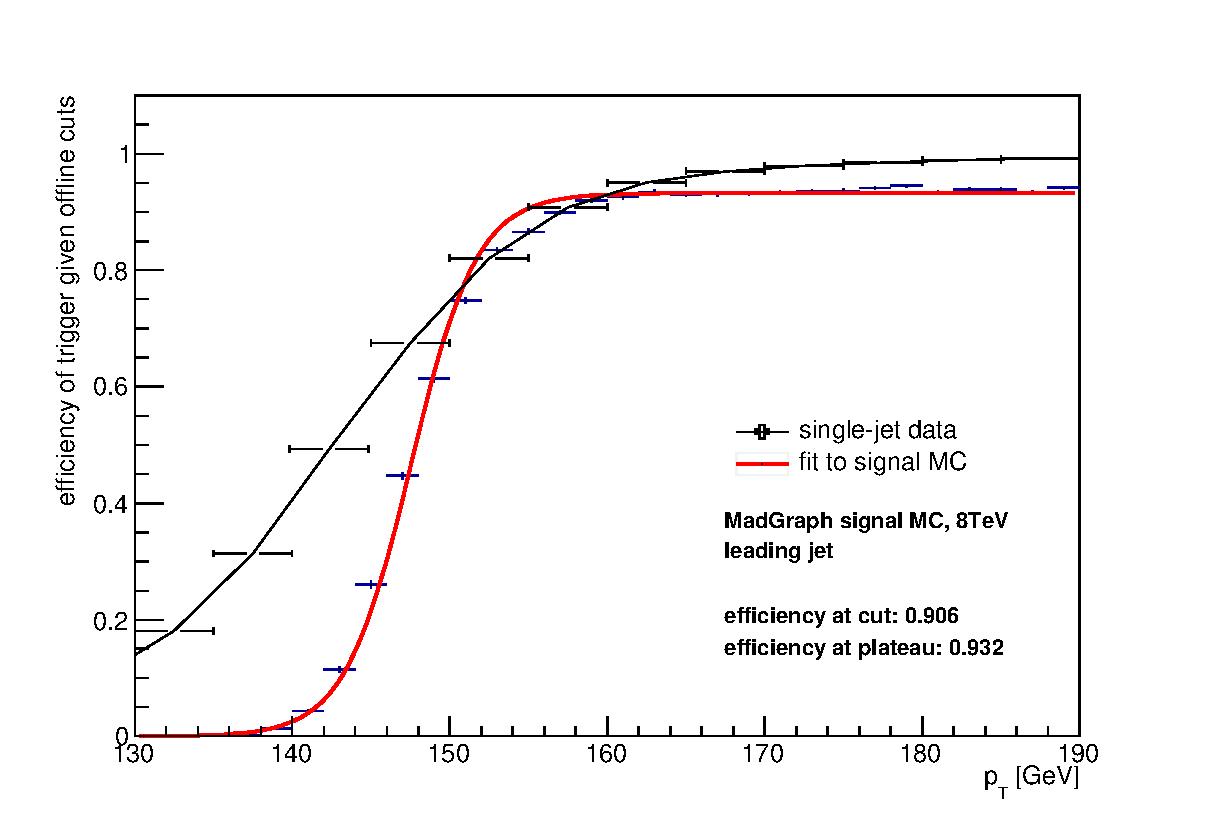
\includegraphics[width=\textwidth]{Systematics/images/jet0_trigger_turn_on_all_j35.eps}\end{subfigure}
%  \begin{subfigure}[sub-leading jet, $m_{A}=400$ GeV]{0.45\textwidth}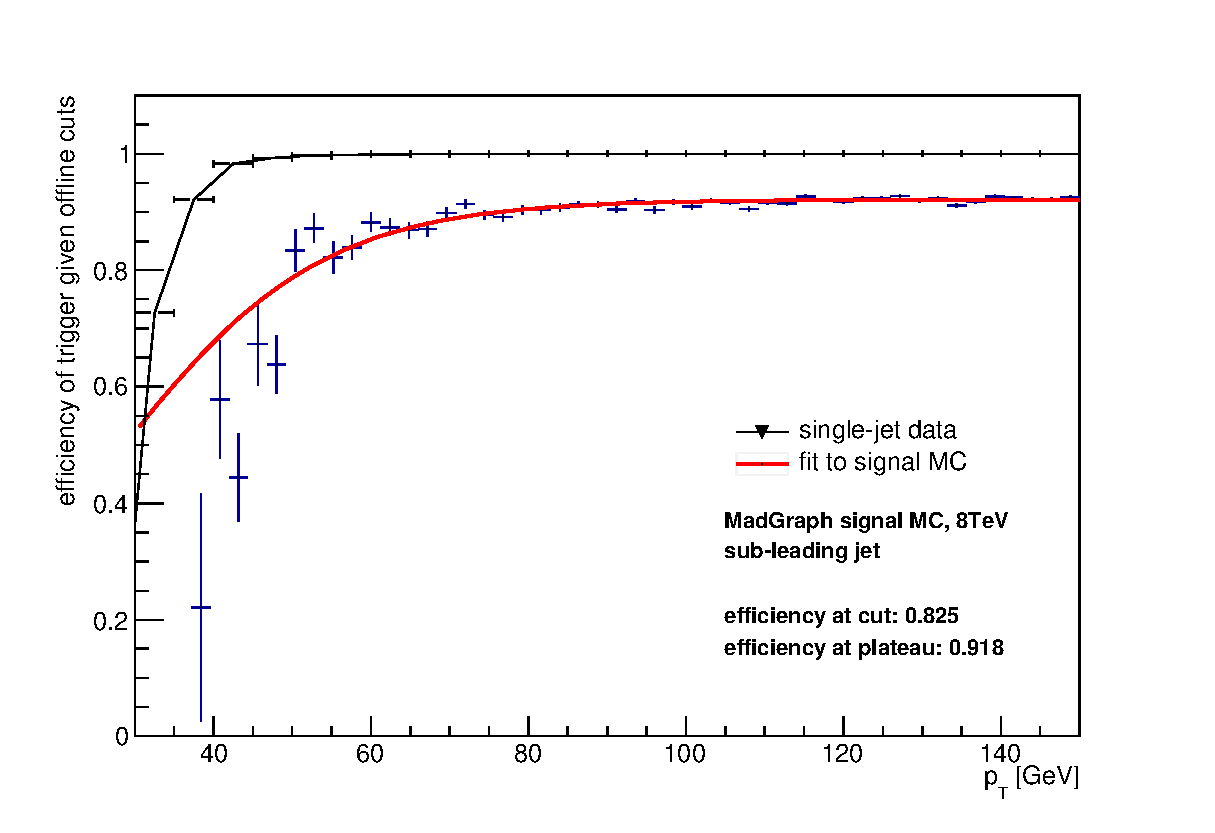
\includegraphics[width=\textwidth]{Systematics/images/jet1_trigger_turn_on_all_j35.eps}\end{subfigure}
%  \begin{subfigure}[leading jet, $m_{A}=450$ GeV]{0.4\textwidth}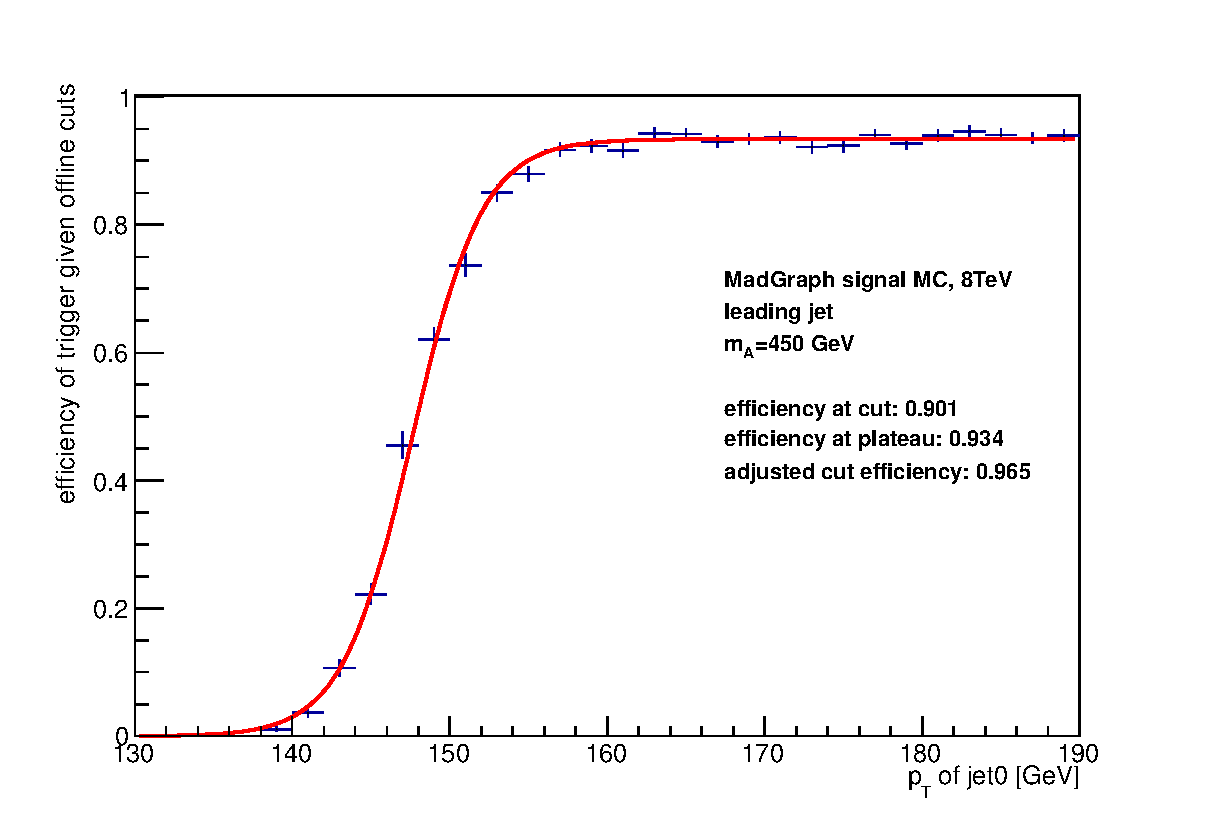
\includegraphics[width=\textwidth]{Systematics/images/jet0_trigger_turn_on_bAbb_450_j35.eps}\end{subfigure}
%  \begin{subfigure}[sub-leading jet, $m_{A}=450$ GeV]{0.4\textwidth}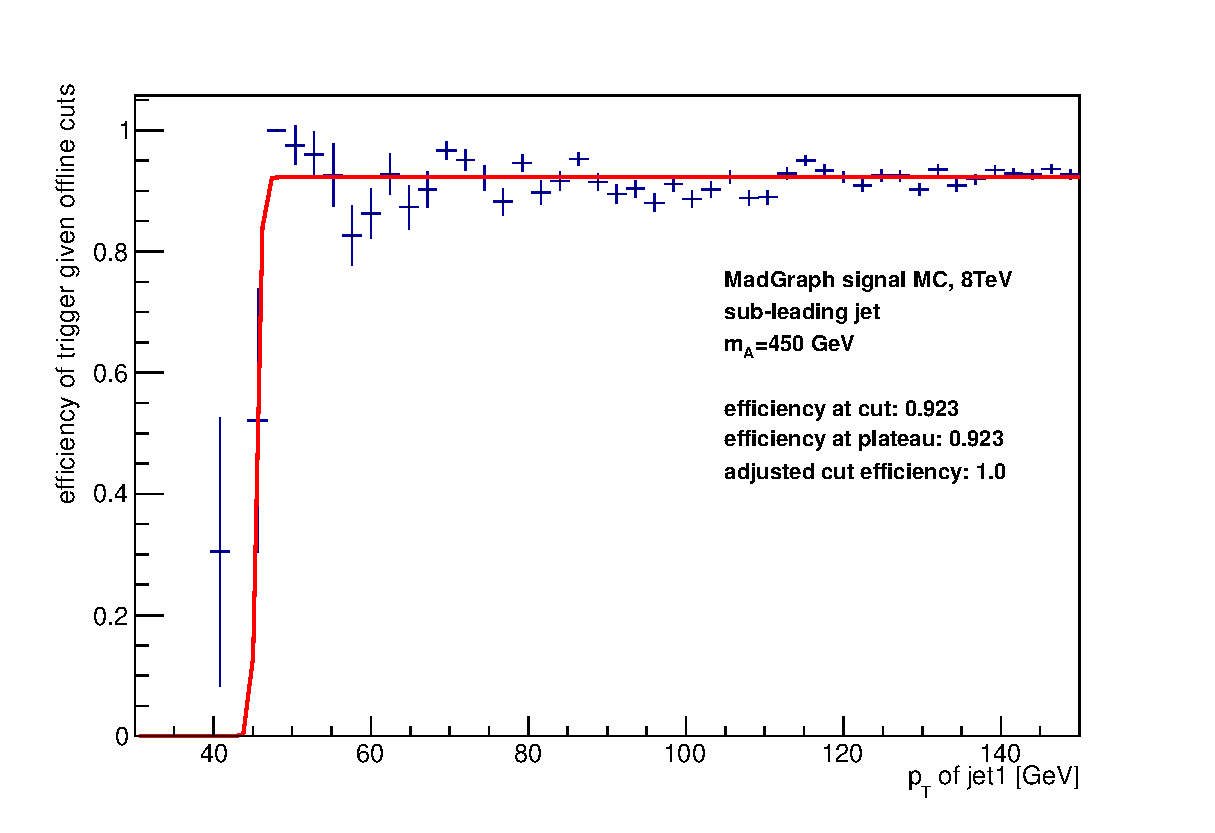
\includegraphics[width=\textwidth]{Systematics/images/jet1_trigger_turn_on_bAbb_450_j35.eps}\end{subfigure}
%  \begin{subfigure}[leading jet, $m_{A}=500$ GeV]{0.4\textwidth}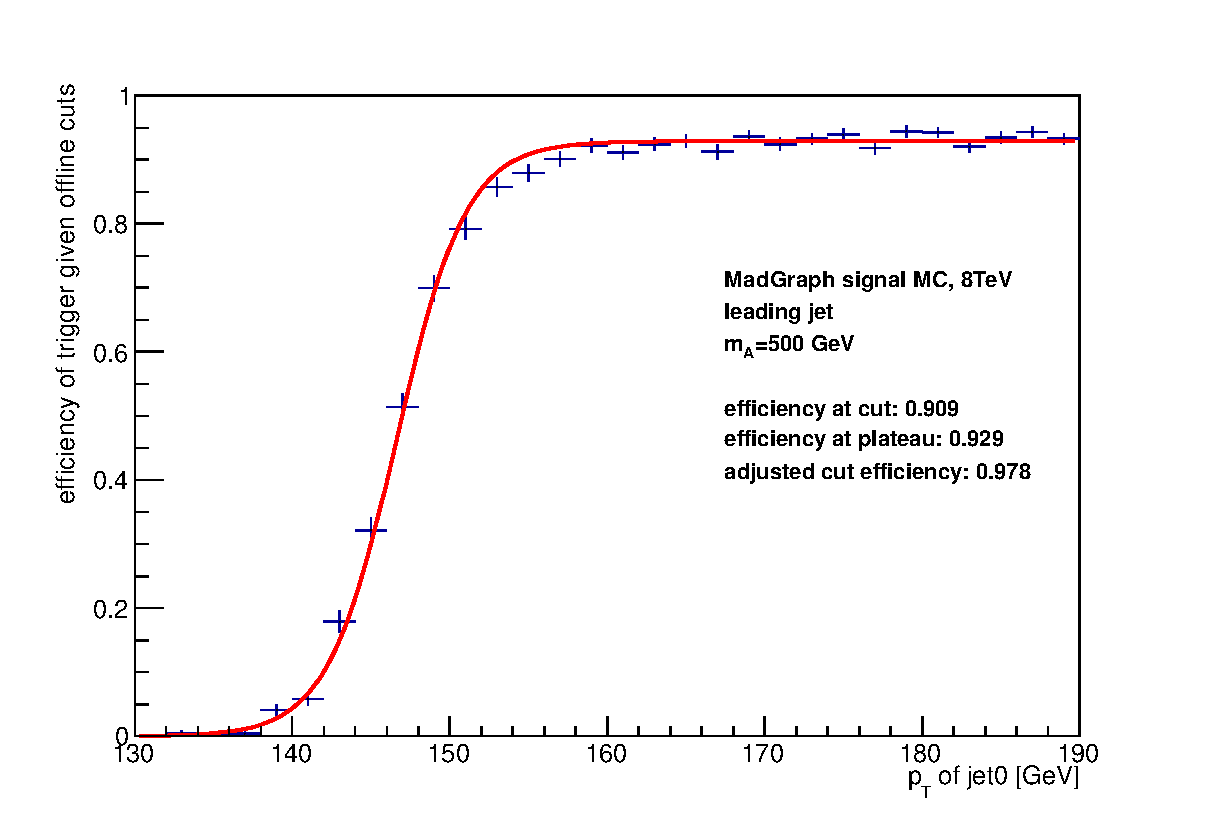
\includegraphics[width=\textwidth]{Systematics/images/jet0_trigger_turn_on_bAbb_500_j35.eps}\end{subfigure}
%  \begin{subfigure}[sub-leading jet, $m_{A}=500$ GeV]{0.4\textwidth}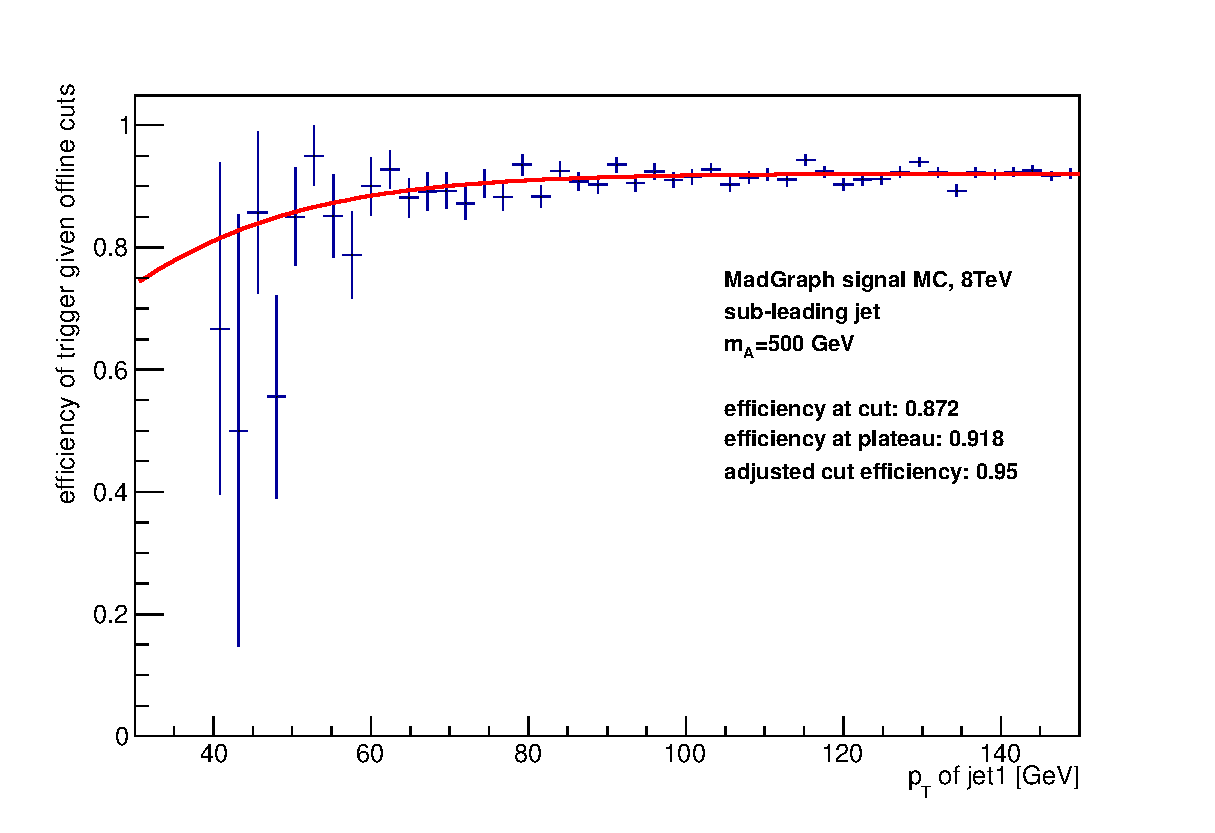
\includegraphics[width=\textwidth]{Systematics/images/jet1_trigger_turn_on_bAbb_500_j35.eps}\end{subfigure}
%  \begin{subfigure}[leading jet, $m_{A}=550$ GeV]{0.4\textwidth}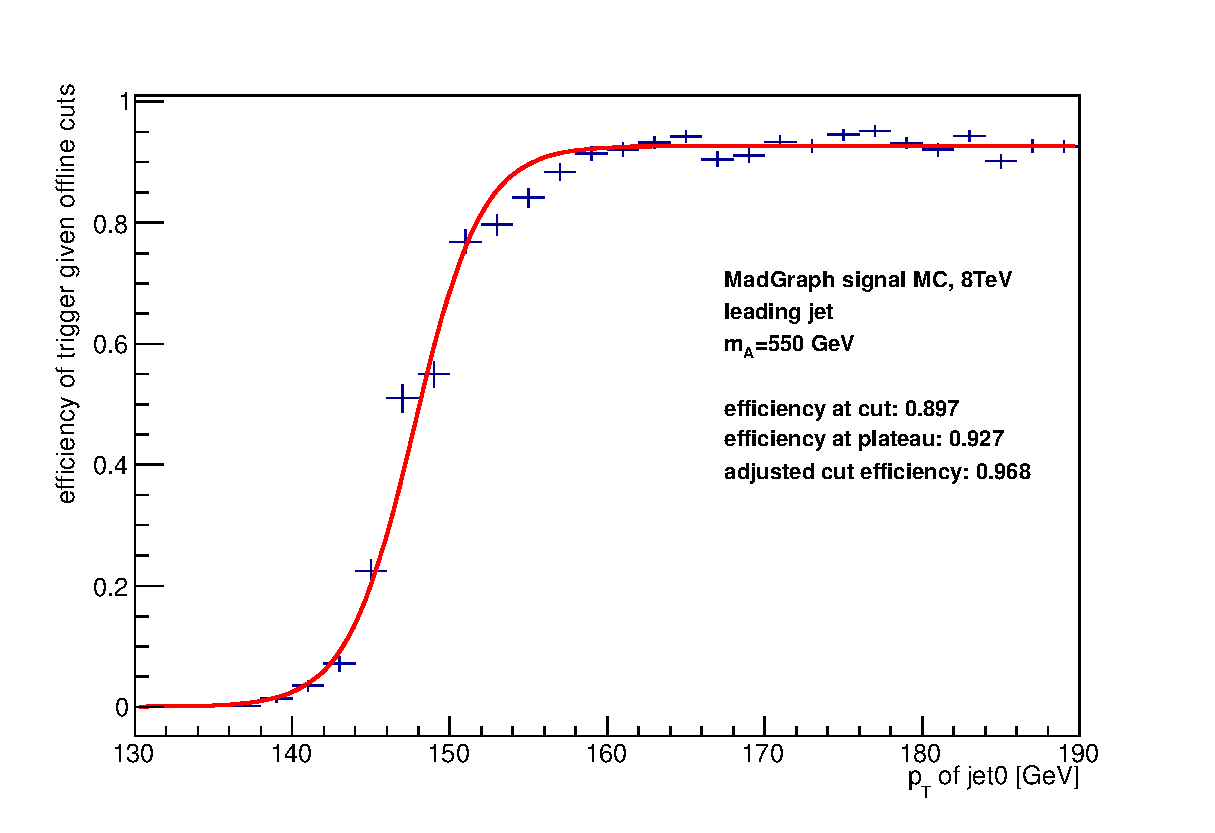
\includegraphics[width=\textwidth]{Systematics/images/jet0_trigger_turn_on_bAbb_550_j35.eps}\end{subfigure}
%  \begin{subfigure}[sub-leading jet, $m_{A}=550$ GeV]{0.4\textwidth}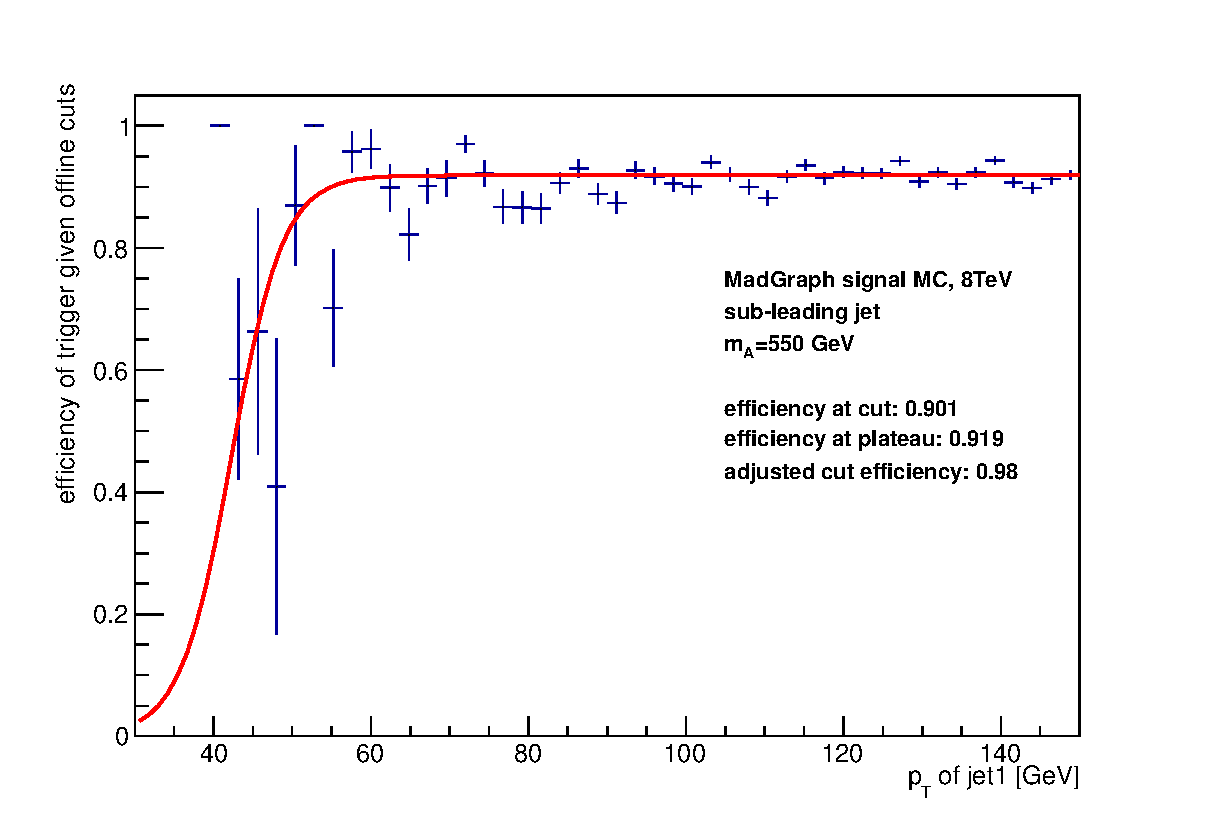
\includegraphics[width=\textwidth]{Systematics/images/jet1_trigger_turn_on_bAbb_550_j35.eps}\end{subfigure}
  \caption{The $p_T$ turn-on curves for the trigger for signal MC and data.
  Although this search uses a multi-object trigger, in which several conditions 
  must simultaneously be true for a trigger acceptance, tight offline cuts can be used to isolate the effect 
  of a single jet's $p_T$ on the efficiency.  The signal curve is fit with a
  logistic function, which is evaluated at a given cut point to extract the trigger efficiency at that point, and to 
  adjust for any residual effects of other trigger objects that affect the efficiency. \label{fig:trigger_turn_on_1}}
    \end{center}
\end{figure}


%\begin{figure}[phtb!]
%  \begin{center}
%  \begin{subfigure}[leading jet, $m_{A}=600$ GeV]{0.4\textwidth}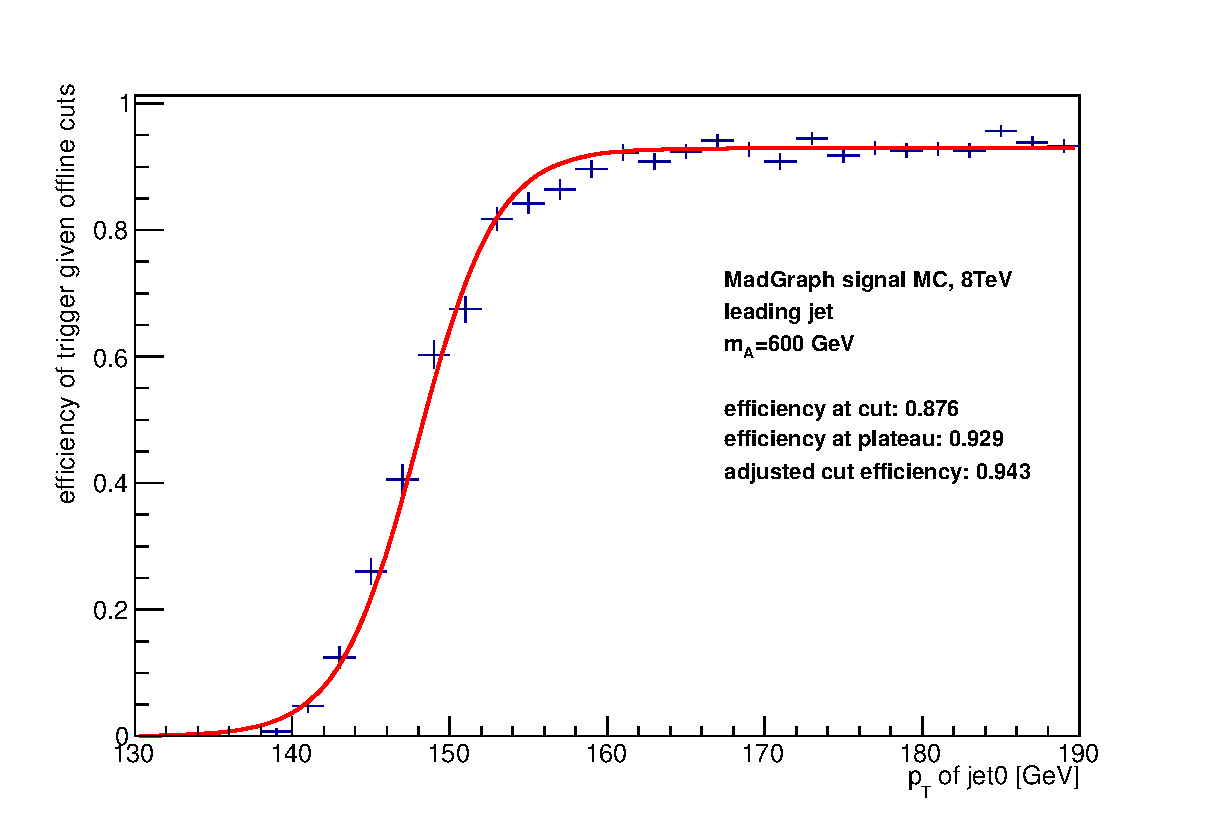
\includegraphics[width=\textwidth]{Systematics/images/jet0_trigger_turn_on_bAbb_600_j35.eps}\end{subfigure}
%  \begin{subfigure}[sub-leading jet, $m_{A}=600$ GeV]{0.4\textwidth}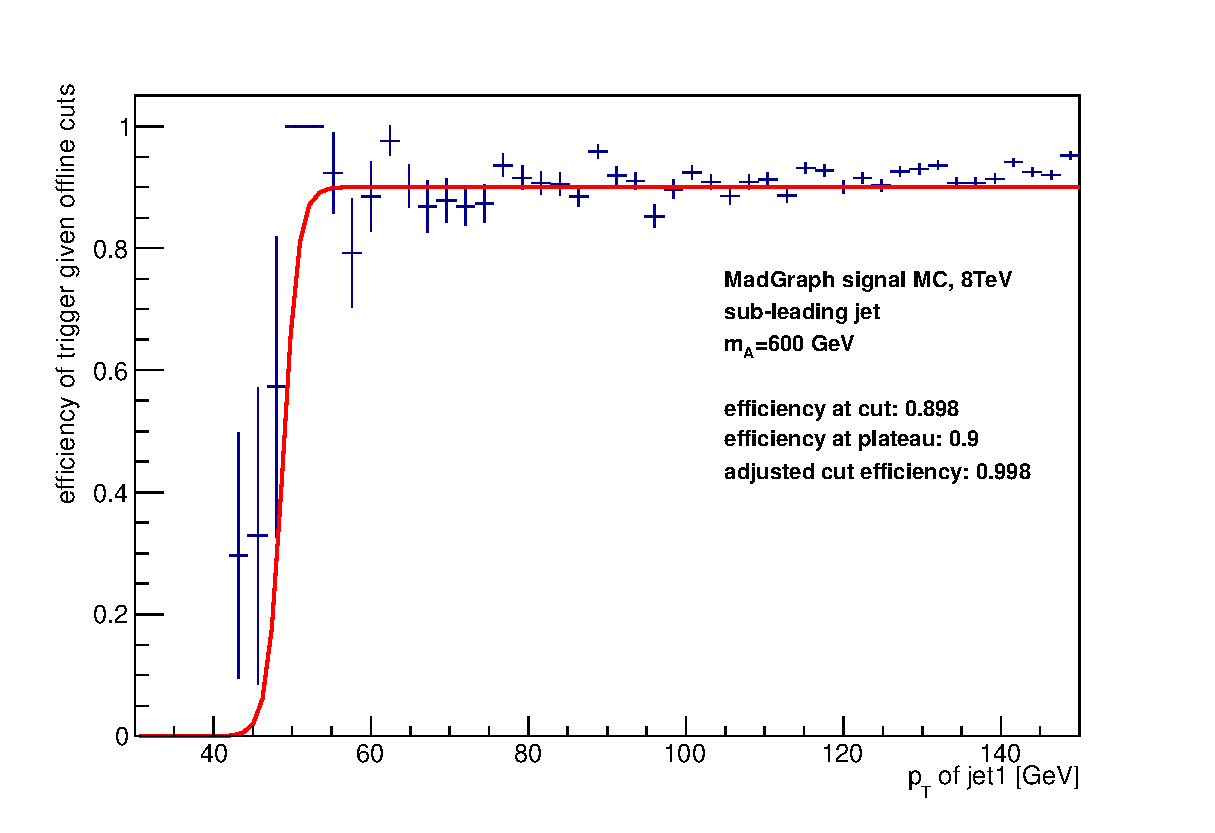
\includegraphics[width=\textwidth]{Systematics/images/jet1_trigger_turn_on_bAbb_600_j35.eps}\end{subfigure}
%  \begin{subfigure}[leading jet, $m_{A}=650$ GeV]{0.4\textwidth}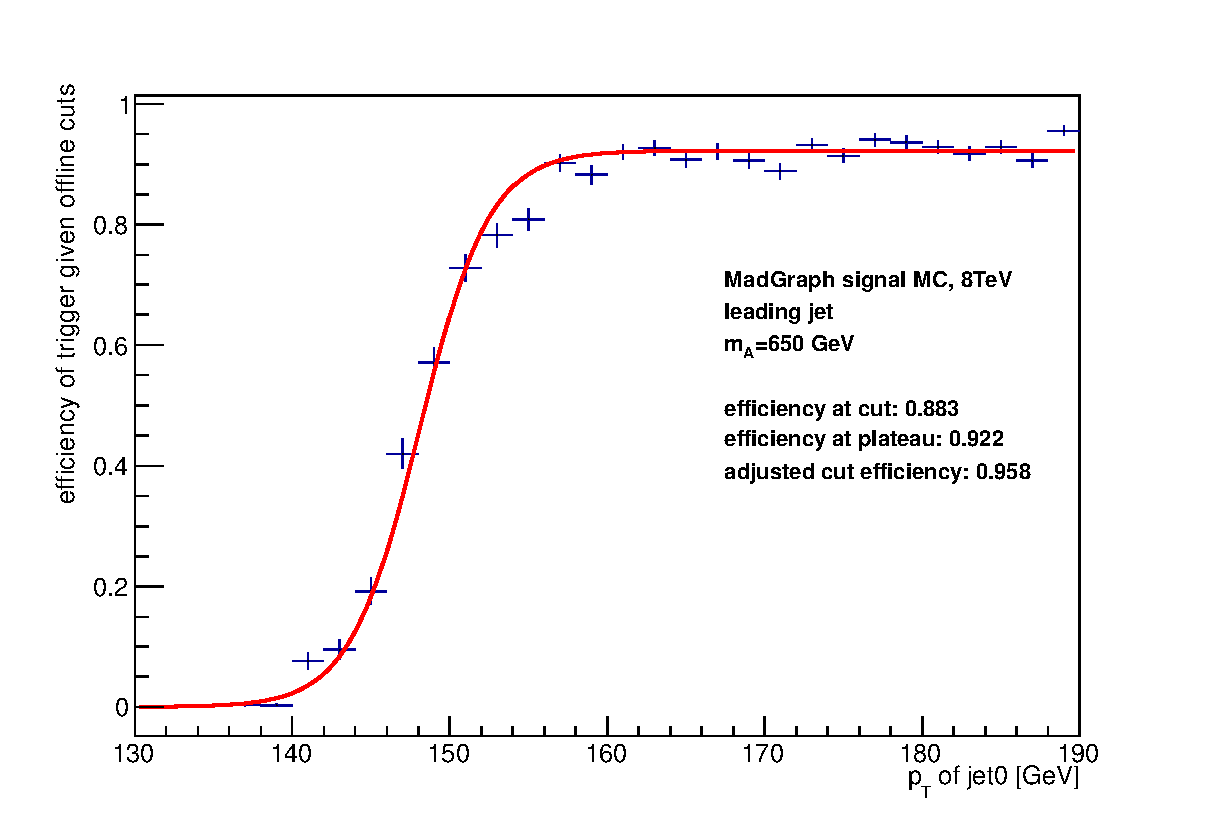
\includegraphics[width=\textwidth]{Systematics/images/jet0_trigger_turn_on_bAbb_650_j35.eps}\end{subfigure}
%  \begin{subfigure}[sub-leading jet, $m_{A}=650$ GeV]{0.4\textwidth}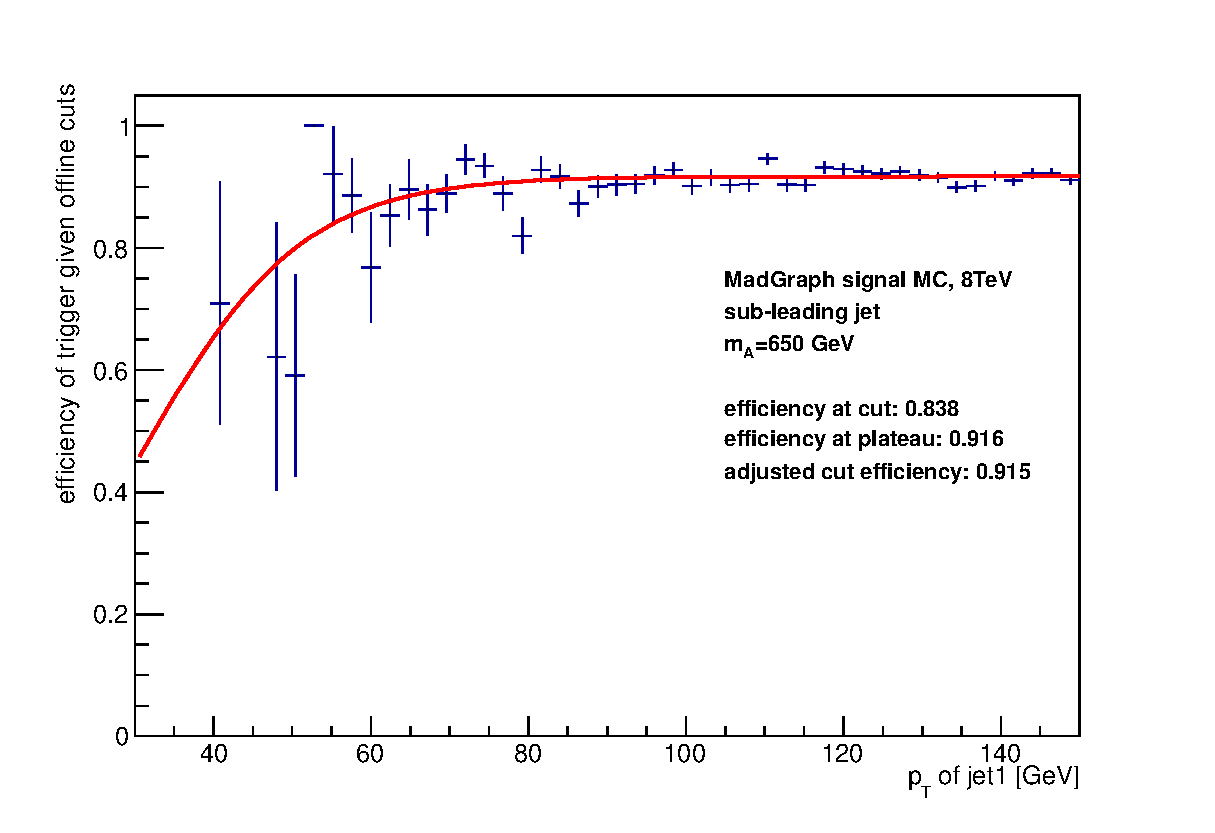
\includegraphics[width=\textwidth]{Systematics/images/jet1_trigger_turn_on_bAbb_650_j35.eps}\end{subfigure}
%  \begin{subfigure}[leading jet, $m_{A}=700$ GeV]{0.4\textwidth}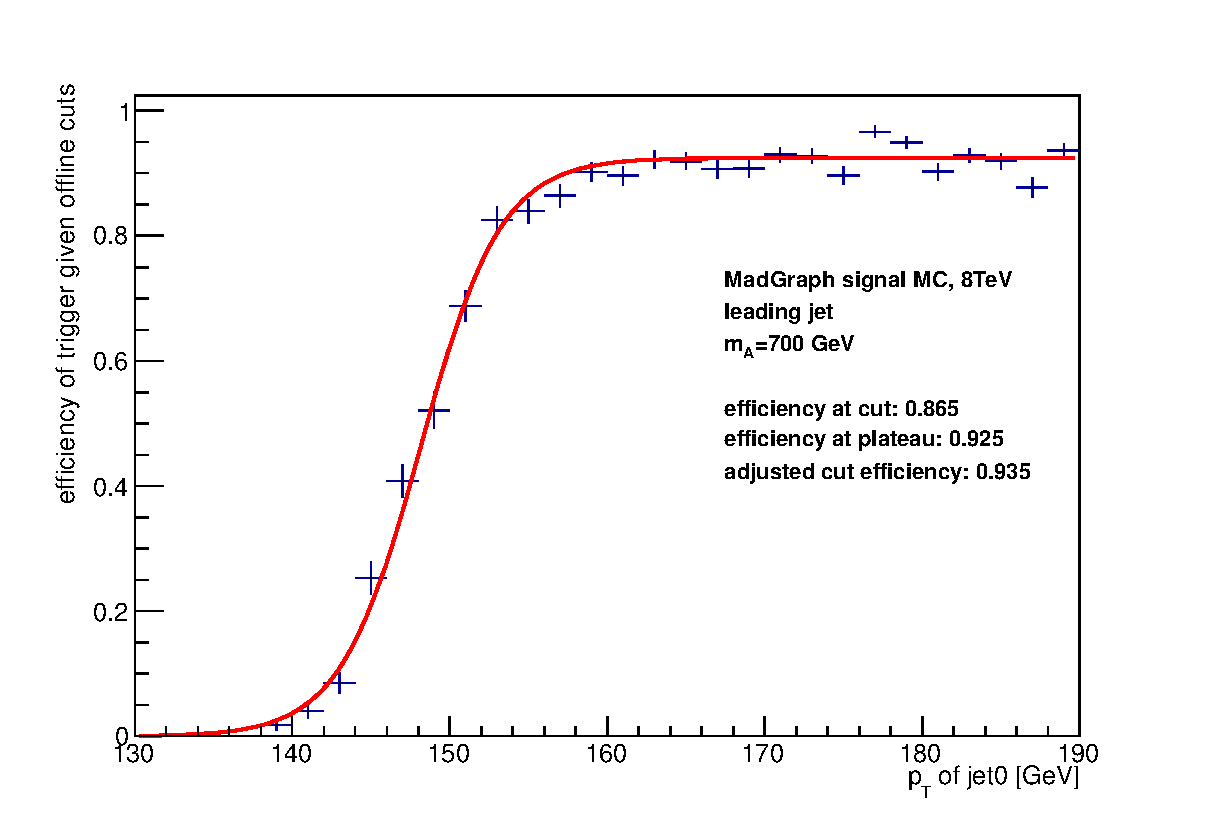
\includegraphics[width=\textwidth]{Systematics/images/jet0_trigger_turn_on_bAbb_700_j35.eps}\end{subfigure}
%  \begin{subfigure}[sub-leading jet, $m_{A}=700$ GeV]{0.4\textwidth}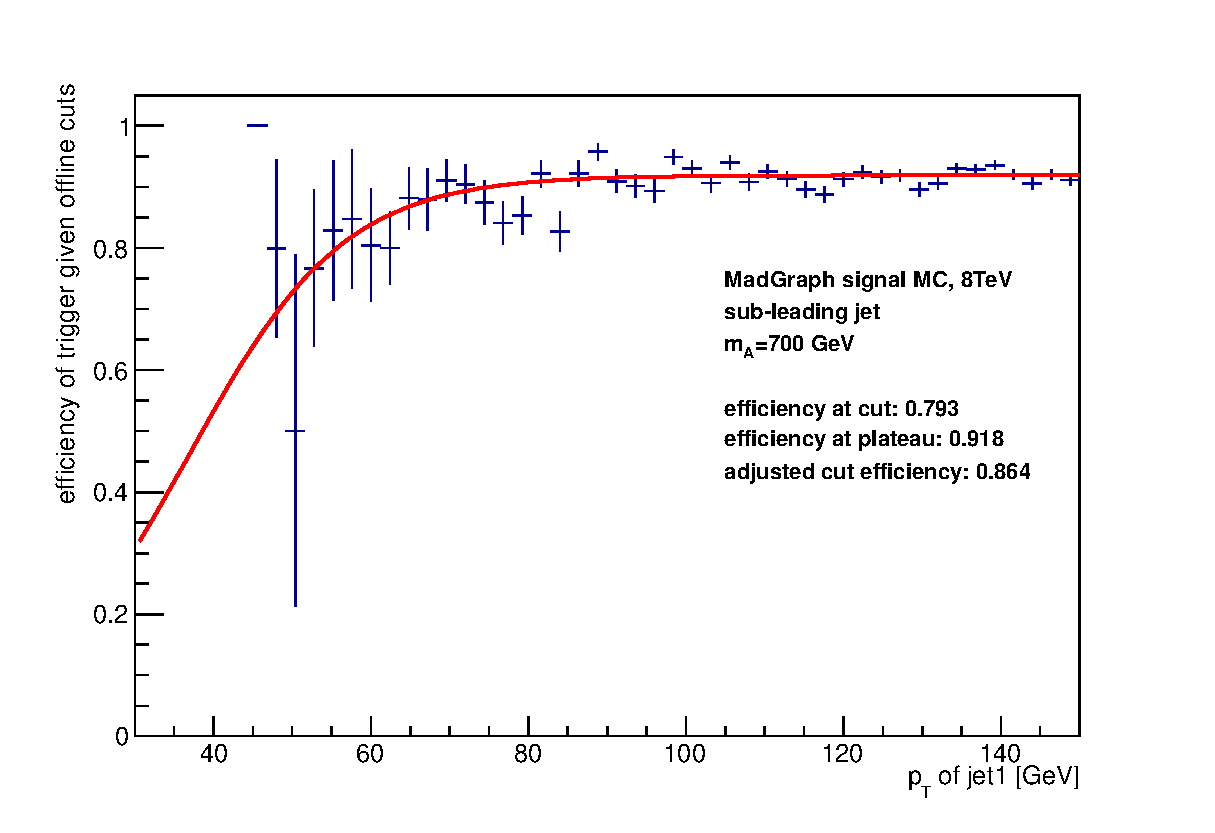
\includegraphics[width=\textwidth]{Systematics/images/jet1_trigger_turn_on_bAbb_700_j35.eps}\end{subfigure}
%  \begin{subfigure}[leading jet, $m_{A}=800$ GeV]{0.4\textwidth}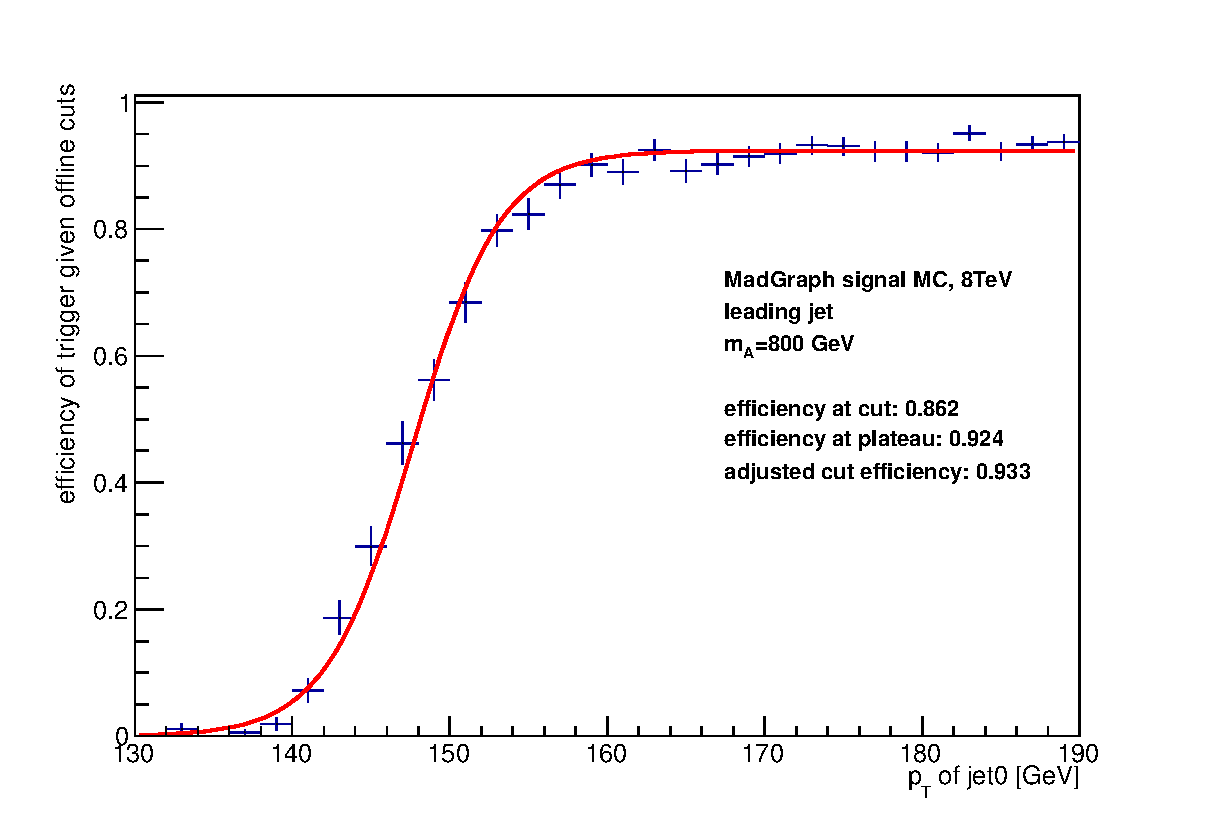
\includegraphics[width=\textwidth]{Systematics/images/jet0_trigger_turn_on_bAbb_800_j35.eps}\end{subfigure}
%  \begin{subfigure}[sub-leading jet, $m_{A}=800$ GeV]{0.4\textwidth}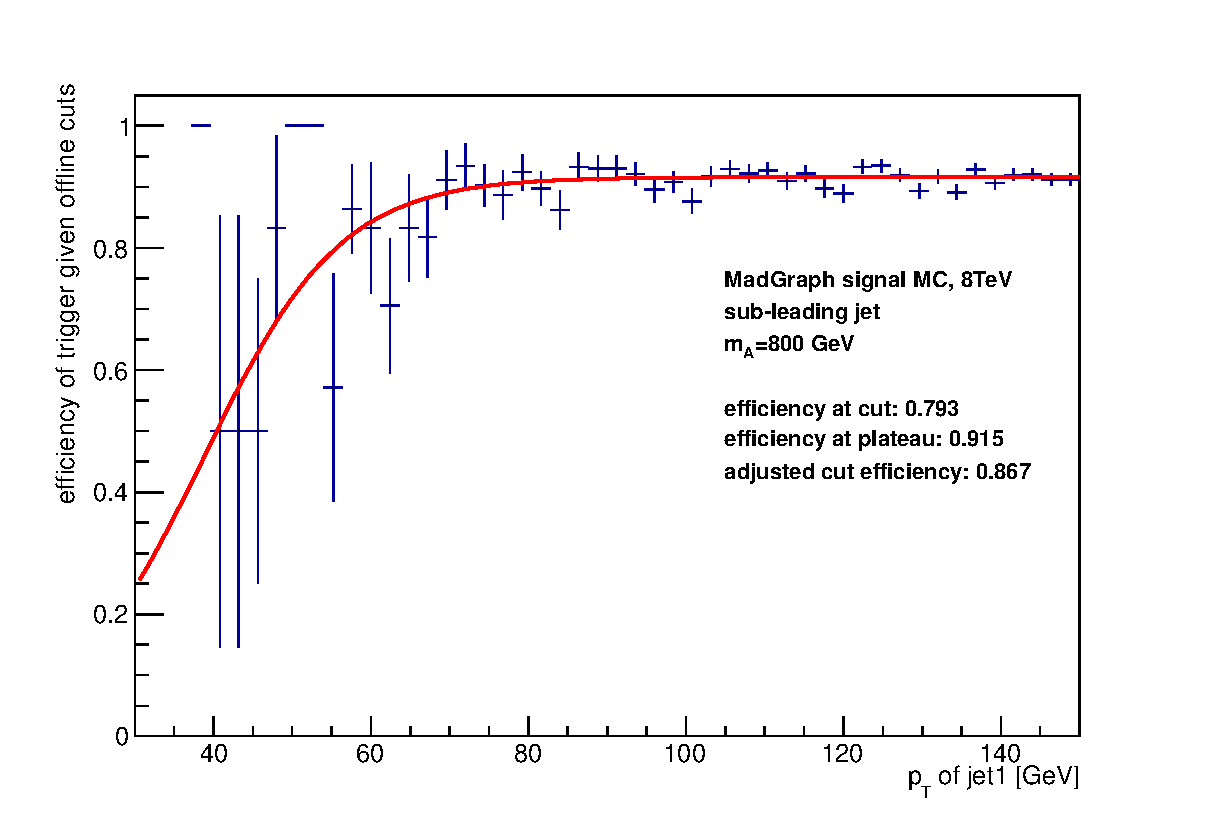
\includegraphics[width=\textwidth]{Systematics/images/jet1_trigger_turn_on_bAbb_800_j35.eps}\end{subfigure}
%  \caption{The $p_T$ turn-on curves for the trigger for signal mass points 600-800 GeV.
%  Although this search uses a multi-object trigger, in which several conditions 
%  must simultaneously be true for a trigger acceptance, tight offline cuts can be used to isolate the effect 
%  of a single jet's $p_T$ on the efficiency.  The curves are fit 
%  with logistics, which are then used to extract the efficiency at the offline cut point, and to 
%  adjust for any residual effects of other trigger objects that affect the efficiency. \label{fig:trigger_turn_on_1}}
%    \end{center}
%\end{figure}



\section{Jet Energy Uncertainties} 
\label{sec:jes}
Hadronic particles fragment via QCD in the ATLAS detector, leaving deposits of 
energy in the calorimeters that must be clustered and reconstructed into jets.  The
observed jets then need some correction so that, on average, the reconstructed
jet energy corresponds to the energy of the associated stable particles.  The
calibration for this correction, called jet energy scale (JES), is calculated using MC simulations and then checked
in data.  The residual uncertainty on the JES is then a systematic 
error on the analysis.

There are a number of sources of JES uncertainty, each of which has an associated error.
All the sources are listed here for completeness, but some are not used for reasons
as noted:
\begin{itemize}
    \item 6 nuisance parameters from in-situ analyses (Z+jet balance, photon+jet balance, and
    multi-jet balance) that are reduced from an original list of 60 that encompasses effects
    such as uncertainties in calorimeter response, the JES calibration method, and modelling
    in Monte Carlo generators
    %\item 2 nuisance parameters associated with flavor composition and flavor response (not used, see next item)
    \item 2 nuisance parameters from $\eta$ intercalibration
    \item 4 nuisance parameters associated with pileup (relative offsets for NPV and $\mu$,
    the $p_T$ of the pileup, and the $\rho$\footnote{in this context, $\rho$ refers to the average energy
    density from pileup throughout the calorimeter} topology)
    \item 1 nuisance parameter that quantifies the flavor composition and flavor
    response associated with $b$-jets
    %\item 1 nuisance parameter associated with MC non-closure (not used since this 
    %is needed to correct non-MC12a samples, but the signal MC was generated as part of MC12a)
    %\item 1 nuisance parameter for punch-through jets (not used because the signal MC
    %was generated using AFII for detector simulation)
\end{itemize} 

The jet energy scale and its associated uncertainties are estimated using
in situ and test-beam-based measurements of isolated hadron response \cite{jes}.  The systematic
errors are integrated into the analysis via 14 independent variations, which are multiplicative factors applied to the jet
4-vectors and then the adjusted 4-vectors are run through the analysis framework.
The effect of the jet energy scale varies depending on the signal mass
point, from about 3\% per variation at 450 GeV to $<$1\% at 800 GeV.  Summing over
all variations gives approximately an 11\% JES uncertainty at 450 GeV (the uncertainties
are summed in quadrature, since they are independent) down to about 4\% at 800 GeV.

%\begin{table}
%    \scriptsize
%    \begin{tabular}{c c c c c c c c c } \hline \hline
%    JES Systematic & 400 GeV & 450 GeV & 500 GeV & 550 GeV & 600 GeV & 650 GeV & 700 GeV & 800 GeV\\ \hline
%    in-situ 1 & & & & & & & & \\
%    in-situ 2 & & & & & & & & \\
%    in-situ 3 & & & & & & & & \\
%    in-situ 4 & & & & & & & & \\
%    in-situ 5 & & & & & & & & \\
%    in-situ 6 & & & & & & & & \\
%    inter-calib model & & & & & & & &  \\
%    inter-calib stat & & & & & & & & \\
%    no. primary vertices & & & & & & & & \\
%    no. interactions pre-beamspot & & & & & & & & \\
%    pileup & & & & & & & & \\
%    rho topology (jet area) & & & & & & & &  \\
%    $b$-jet response model & & & & & & & & \\
%    \end{tabular}
%\end{table}



%Similarly, the jet energy resolution is measured using dijet balance measurements and 
%a dijet bisection technique \cite{jer}, in
%order to quantify the jet resolution or $\sigma p_T/p_T$.  Data and MC simulations are 
%found to agree to within 14\% for central ($|y|<$2.8) jets with $p_T$ betweeen
%20 and 80 GeV.


\section{$b$-Tagging Scale Factors}
\label{sec:SF}
Although every effort is made to accurately simulate the production rates and
kinematic properties of $b$-quarks, as well as the performance of the ATLAS
detector, it is difficult to imagine that Monte Carlo simulation perfectly represents
the $b$-tagging efficiencies that might be found in data.  At the same time, it
is challenging to derive pure data-driven samples of $b$, $c$ and light jets to which
the b-tagging can then be applied, and used to derive the efficiencies:

    \begin{equation}
        eff_{b,c,light}=\frac{number\ of\ tagged\ b,\ c,\ light}{number\ of\ truth\ b,\ c,\ light}
    \end{equation}

Scale factors are computed by the flavor tagging performance group to quantify the
difference between the data and MC efficiencies.

    \begin{equation}
        eff_{data}=eff_{MC}\times SF_{data}
    \end{equation}


The scale factors are applied as event weights to the MC events, where the value
of the scale factor depends on the $p_T$, $\eta$, $b$-tagging working point, 
and truth flavor of the jet under examination.  
When there are multiple jets being examined for $b$-tags in a single
event, the net event weight is a product of all the relevant scale factors.
In this analysis, since only the first 5 jets are relevant for determining 
whether an event passes the analysis cuts or which $b$-tag category ($bbb$, 
$bbloose$, or $bbanti$), no scale factors are applied for jets that are 6th
or lower in the $p_T$ hierarchy of an event.

\subsection{Offline $b$-Tagging}
The scale factors are calculated by comparing the $b$-tagging efficiency computed 
in MC to the efficiency measured in carefully curated data samples, where the truth
flavor contents of the data are relatively well-known \cite{b-tagging}.  For the $b$-jet
scale factors, a sample of $t\bar{t}$ events is used for the data component; for 
$c$-jets, the calibration is done with $D^*$ events.

The scale factors are used to correct the MC $b$-tagging performance back to the $b$-tagging
behavior seen in data, but the calibration process can introduce systematic uncertainties
that have to be quantified and propagated through to the final result.  The $b$-tagging
systematics are computed and applied using a method called the eigenvector method.
The eigenvector method is used to derive a set of independent variations of the data-MC scale
factors, in such a way to take the full covariance matrix of the calibration measurements
into account, including correlations among working points and different jet $p_{T}$ regions.
For further explanation of the eigenvector method please see section 2.3 of \cite{VHBTagging}. 

The differences between the eigenvector variations and the nominal scale factors
are combined in quadrature separately for each category in $n_{jets}$.  We find that
the effect on the normalization of the signal is 15-19\%, depending on mass point and
$n_{jets}$ category.


\subsection{$b$-Tagging in the Trigger}
The presence of $b$-tagging in the trigger means the sample of data collected for this 
analysis is already enriched in jets that look more $b$-like, which must also 
be taken into account during the calibration process.  The scale factors
are computed separately based on how a jet is tagged (online, offline, or both). 
For each of these permutations, a different scale factor is retrieved (for
example, jets that are tagged offline are separated from their non-tagged counterparts
before the online scale factors are computed).  Then the scale factors are combined
for an overall event weight as usual.  

When we examine the online scale factors for systematic uncertainties, the most
important errors are the errors on jets that are $b$-tagged offline as well as online,
since that describes the jets that are most important when identifying signal events. 
The systematic uncertainties on these scale factors are approximately 4\% per jet, 
and there is not any significant relationship between the $p_T$ of the jet
and the online $b$-tagging uncertainty.  

\begin{figure}
    \center
  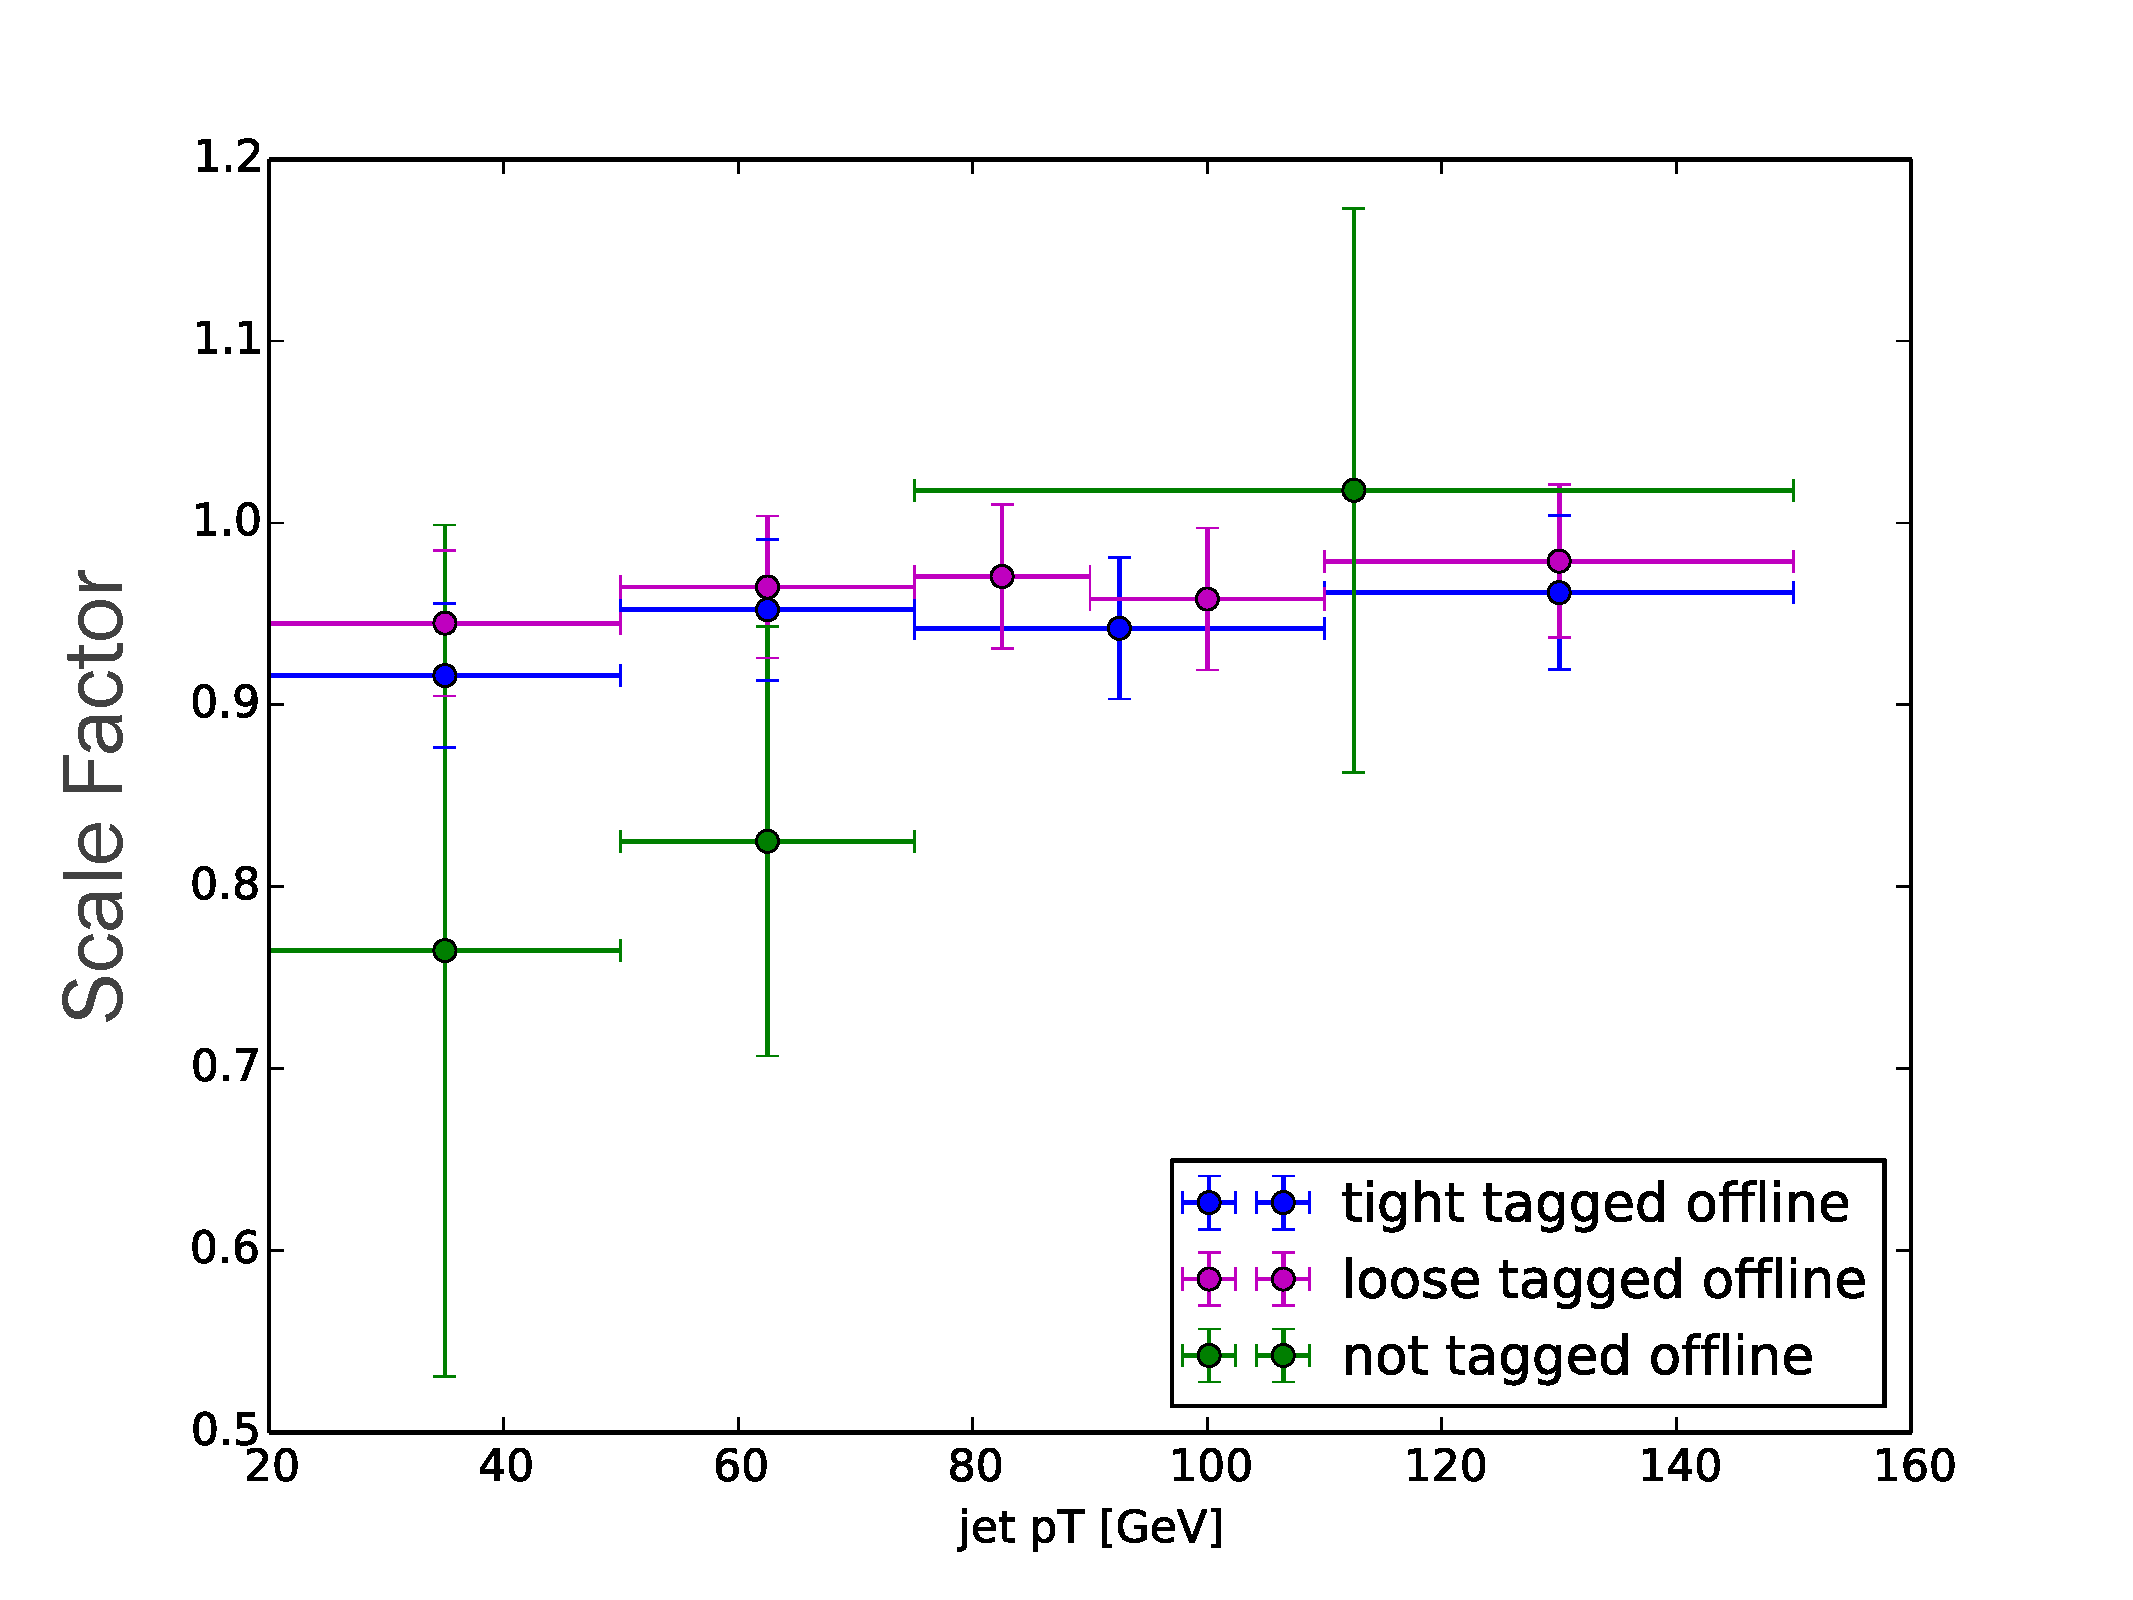
\includegraphics[width=0.85\linewidth]{Systematics/online_SFs.pdf}
  \caption{The online $b$-tagging scale factors as a function of jet $p_T$ for
  jets categorized by how tightly they are tagged offline.  For jets with a $p_T$
  higher than the maximum calibrated $p_T$ point, we apply the scale factor for the 
  highest $p_T$ bin that has a calibration. \label{fig:online_sfs}}    
\end{figure}                                                                                                                        












